\documentclass[11pt,letterpaper]{article}

% Page and text formatting
\usepackage[margin=1in]{geometry}
\usepackage[T1]{fontenc}
\usepackage{lmodern}
\usepackage{microtype}
\usepackage{setspace}
\setstretch{1.10}
\setlength{\parindent}{0pt}
\setlength{\parskip}{0.45em}

% Figures, tables, and SQL
\usepackage{graphicx}
\usepackage{amsmath,amssymb}
\usepackage{array,tabularx}
\usepackage{enumitem}
\usepackage{listings}
\usepackage[table]{xcolor}
\usepackage{placeins}
\usepackage{caption}
\usepackage{float}
\usepackage[hidelinks]{hyperref}
\setlist[itemize]{leftmargin=*,itemsep=0.15em,topsep=0.25em}

\lstdefinestyle{projectSQL}{
    language=SQL,
    basicstyle=\ttfamily\scriptsize,
    keywordstyle=\color{blue!50!black}\bfseries,
    commentstyle=\color{gray!75!black}\itshape,
    stringstyle=\color{teal!60!black},
    breaklines=true,
    breakatwhitespace=false,
    columns=fullflexible,
    keepspaces=true,
    showstringspaces=false,
    frame=single,
    rulecolor=\color{black!30},
    framesep=5pt,
    aboveskip=0.5em,
    belowskip=0.5em
}
\lstset{style=projectSQL}

\title{Supermarket Chain Database Web Application\\COSC 3380 --- Project Report}
\author{Matthew Dulworth \and Javier Puentes Leiva}
\date{Fall 2026}

\begin{document}
\maketitle

\section{Introduction}

This project implements a database-backed web application for a chain of 100 supermarkets across multiple states. It simulates product sales, store-specific inventory, tax calculations, and cash or card payments. The application uses PostgreSQL for data storage, Node.js and Express for the backend, and HTML and JavaScript for the frontend.

The supermarket and bank are separate databases. The web interface supports customer checkout, back-office reports, database administration, random checkout simulation, and concurrent customers. Transactions, row locking, and two-phase commit help keep purchases, inventory, and card payments consistent.

\section{Database Design and Final ER Model}

\subsection{Database Structure}

The supermarket database contains seven related tables; the bank database contains one. Their responsibilities are summarized below.

\begin{center}
\small
\begin{tabularx}{\textwidth}{@{}>{\bfseries}p{0.24\textwidth}X@{}}
\hline
Table & Purpose \\ \hline
Tax & State sales tax rates \\
Department & Product categories \\
Store & Store locations, contact details, and aisles \\
Item & Product SKU, department, and tax/weight flags \\
Inventory & Product price, stock, and aisle by store \\
Store Transaction & Purchase date, store, payment method, and total \\
Item Sale & Products, quantities, and unit prices within each purchase \\
Account (bank) & Account numbers and balances \\ \hline
\end{tabularx}
\end{center}

\subsection{Final ER Model}

Figure~\ref{fig:final-er} shows the final supermarket ER model, which contains seven tables. The main one-to-many relationships are: one state tax record can apply to multiple stores; one store can have multiple transactions; and one department can contain multiple items. Each transaction belongs to one store, each item belongs to one department, and each store references one state tax record.

The \texttt{Inventory} table connects stores and items, allowing the same product to have different prices, stock quantities, and aisle locations at different stores. Its composite primary key, \texttt{(sku, store\_id)}, uniquely identifies each store--product combination. Similarly, \texttt{Item Sale} connects transactions and items, recording the quantity and unit price for each purchased product. Its composite primary key is \texttt{(transaction\_id, sku)}. These two tables implement the many-to-many relationships between stores and items, and between transactions and items.

Foreign keys enforce the relationships shown in the diagram, while \texttt{tax\_exempt} and \texttt{priced\_by\_weight} in \texttt{Item} determine how products are handled during checkout. A completed purchase consists of one transaction record and its corresponding item-sale records.

\begin{figure}[H]
    \centering
    \includegraphics[width=0.95\textwidth,height=0.49\textheight,keepaspectratio]{v3.png}
    \caption{Final Supermarket ER Model}
    \label{fig:final-er}
\end{figure}

The bank is modeled separately with the \texttt{Account} table (Figure~\ref{fig:bank-er}), whose primary key is \texttt{account\_number} and whose \texttt{balance} stores available funds. For card purchases, \texttt{store\_transaction.account\_id} identifies the bank account; for cash purchases, it is null. Because the databases are separate, this association is checked by the application rather than a cross-database foreign key.

\begin{figure}[H]
    \centering
    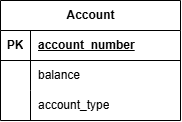
\includegraphics[width=0.38\textwidth,height=0.16\textheight,keepaspectratio]{bank.png}
    \caption{Bank Database ER Model}
    \label{fig:bank-er}
\end{figure}
\FloatBarrier

\section{Receipt Analysis}

Five receipts from H-E-B, Target, Tesco, Trader Joe's, and Whole Foods Market were examined to identify the fields needed for checkout and sales records. The original receipts appear in Appendix~\ref{app:receipts}.

\begin{center}
\small
\begin{tabularx}{\textwidth}{@{}>{\bfseries}p{0.19\textwidth}X@{}}
\hline
Receipt & Relevant observation \\ \hline
H-E-B & Weighted chestnuts, coupon savings, and card payment \\
Target & Multiple departments, discounts, and tax classifications \\
Tesco & Items sold by weight, VAT rates, and a different currency \\
Trader Joe's & Unit quantities, item prices, and payment totals \\
Whole Foods & Weighted produce, discounts, and tax details \\ \hline
\end{tabularx}
\end{center}

These examples informed the \texttt{Item}, \texttt{Inventory}, \texttt{Item Sale}, \texttt{Store Transaction}, and \texttt{Tax} tables. The design captures product identity, quantity or weight, price, transaction time, payment type, and applicable tax. Discounts, multiple tax rates within one location, foreign currencies, and metric-unit checkout are outside the implemented scope.

\section{Normalization and Physical Database Design}

\subsection{Normalization and Functional Dependencies}

The database was designed to satisfy 3NF and, where possible, BCNF. Each table was analyzed using its functional dependencies to identify partial and transitive dependencies. The identified dependencies have candidate keys as determinants, supporting BCNF under the modeled dependencies.



Certain attributes were intentionally stored for practical purposes. For example, the \texttt{total\_amount} attribute in the \texttt{store\_transaction} table stores the final amount charged to the customer, even though it can be calculated from purchased items and applicable taxes. This introduces redundancy across related tables but improves reporting efficiency and preserves the recorded transaction total.

Similarly, the \texttt{unit\_price} attribute in the \texttt{item\_sale} table preserves historical purchase prices when inventory prices change. Unlike the derived total, this historical attribute does not inherently violate normalization.



\renewcommand{\arraystretch}{1.16}
\begin{center}
\footnotesize
\begin{tabularx}{\textwidth}{@{}>{\bfseries}p{0.23\textwidth}>{\raggedright\arraybackslash}X@{}}
\hline
Relation & Functional dependency \\ \hline
Tax & \texttt{state\_code} $\rightarrow$ \texttt{tax\_rate} \\
Department & \texttt{department\_id} $\rightarrow$ \texttt{name} \\
Store & \texttt{store\_id} $\rightarrow$ address, state, phone, aisles \\
Item & \texttt{sku} $\rightarrow$ name, department, tax and weight flags \\
Inventory & \texttt{(sku, store\_id)} $\rightarrow$ price, stock, aisle \\
Store Transaction & \texttt{transaction\_id} $\rightarrow$ store, account, time, total, payment method \\
Item Sale & \texttt{(transaction\_id, sku)} $\rightarrow$ quantity, unit price \\
Account & \texttt{account\_number} $\rightarrow$ balance \\ \hline
\end{tabularx}
\end{center}




\subsection{Physical Tables and Constraints}

The final ER model was implemented as relational tables in PostgreSQL. The main transaction-related tables and their mappings are summarized below.

\begin{center}
\small
\begin{tabularx}{\textwidth}{@{}p{0.23\textwidth}X@{}}
\hline
Table & Relational Mapping \\ \hline

\texttt{store\_transaction} &
Primary key: \texttt{transaction\_id}.
Foreign key: \texttt{store\_id}.
Records each purchase and its payment information. \\

\texttt{item\_sale} &
Composite primary key: \texttt{(transaction\_id, sku)}.
Both attributes are foreign keys, connecting transactions to purchased products. \\

\texttt{inventory} &
Composite primary key: \texttt{(sku, store\_id)}.
Both attributes are foreign keys, connecting products to supermarket locations. \\

\texttt{account} &
Primary key: \texttt{account\_number}.
Stores bank balances in the separate bank database. \\ \hline

\end{tabularx}
\end{center}

Primary keys enforce entity integrity, while foreign keys enforce referential integrity. CHECK constraints prevent negative stock quantities, prices, and bank balances, and restrict transaction payment methods to cash or card.

The complete SQL table definitions are provided in \texttt{ddl.sql} and \texttt{bankddl.sql}, which are submitted separately with the application source code.



\subsection{Indexes}

PostgreSQL automatically indexes primary keys. Six additional indexes were added for inventory lookup, low stock, transaction dates, product sales, and department lookup. Two examples are:

\begin{lstlisting}
CREATE INDEX idx_inventory_store_sku
    ON inventory(store_id, sku);
CREATE INDEX idx_transaction_store_date
    ON store_transaction(store_id, date_and_time DESC);
\end{lstlisting}

The remaining indexes cover \texttt{inventory.quantity\_in\_stock}, \texttt{store\_transaction.date\_and\_time}, \texttt{item\_sale.sku}, and \texttt{item.department\_id}. \texttt{EXPLAIN ANALYZE} confirmed a Bitmap Index Scan using \texttt{idx\_transaction\_store\_date} for a store/date query. PostgreSQL's optimizer chooses when an index is beneficial, using statistics updated by \texttt{ANALYZE}.

\section{Web Application Implementation}

\subsection{Architecture and User Interfaces}

The frontend in \texttt{home.html} sends HTTP requests to the Express API in \texttt{server.js}, which validates inputs and executes parameterized PostgreSQL queries through separate supermarket and bank connection pools. The Customer Checkout tab selects a store, adds unit- or weight-based products to a cart, and processes cash or card purchases.

The Supermarket Backend tab supports table browsing, deletion and regeneration, plus four reports: monthly sales, top-selling items by department, low-stock inventory, and recent transactions. The Bank tab displays account balances and allows account regeneration.


\subsection{Simulation and SQL Tracing}

The frontend supports random and concurrent checkout simulations. The backend executes SQL transactions and uses row locks to protect inventory updates. A tracing system displays executed SQL statements and their execution times in milliseconds, while saving checkout and report traces to \texttt{transaction.sql} and \texttt{query.sql}.


\section{Transaction Processing and ACID Properties}

\subsection{Checkout Transaction}

Each checkout validates the store, SKUs, quantities, and payment method. Inside a PostgreSQL transaction, it locks the selected inventory rows with \texttt{FOR UPDATE}, checks available stock, calculates tax in SQL, inserts a purchase and its item-sale records, and decrements inventory. For card payments, the separate bank transaction deducts funds only when the account has a sufficient balance. Failed checks cause a rollback rather than a partial sale.

The following excerpt shows the main SQL operations executed by \texttt{server.js}; placeholders such as \texttt{\$1} are parameters supplied by the backend, and the inventory operations are repeated for each purchased SKU.

\begin{lstlisting}
-- Supermarket database
BEGIN;
SET LOCAL lock_timeout = '10s';
SELECT inv.price, inv.quantity_in_stock,
       i.tax_exempt, i.priced_by_weight, t.tax_rate
FROM inventory AS inv
JOIN item AS i ON inv.sku = i.sku
JOIN store AS s ON inv.store_id = s.store_id
JOIN tax AS t ON s.state_code = t.state_code
WHERE inv.store_id = $1 AND inv.sku = $2
FOR UPDATE OF inv;

-- Bank database, for card payments only
BEGIN;
UPDATE account
SET balance = balance - $1
WHERE account_number = $2 AND balance >= $1
RETURNING account_number, balance;

-- Supermarket database, after validation and totaling
INSERT INTO store_transaction
    (store_id, account_id, total_amount, payment_method)
VALUES ($1, $2, $3, $4)
RETURNING transaction_id;
INSERT INTO item_sale
    (transaction_id, sku, quantity_sold, unit_price)
VALUES ($1, $2, $3, $4);
UPDATE inventory
SET quantity_in_stock = quantity_in_stock - $1
WHERE store_id = $2 AND sku = $3;
\end{lstlisting}

\subsection{ACID and Two-Phase Commit}

\textbf{Atomicity} is enforced with \texttt{BEGIN}, \texttt{COMMIT}, and \texttt{ROLLBACK}. \textbf{Consistency} is supported by primary/foreign keys, CHECK constraints, stock validation, and sufficient-funds checks. \textbf{Isolation} uses row-level inventory locks, with SKUs processed in sorted order and a 10-second lock timeout. \textbf{Durability} relies on PostgreSQL's committed transactions.

Cash purchases update only the supermarket database and use a normal \texttt{COMMIT}. Card purchases change two databases and therefore use PostgreSQL's two-phase commit. The bank and supermarket transactions are first prepared; after both succeed, they are committed. Prepared-transaction identifiers are generated by the server rather than entered by users. The identifiers below are illustrative: the backend generates a unique ID for each checkout, and the commands run on separate database connections.

\begin{lstlisting}
-- Both connections have already executed BEGIN and DML.
-- Phase 1: prepare both databases
PREPARE TRANSACTION 'checkout-<id>-bank';
PREPARE TRANSACTION 'checkout-<id>-supermarket';
-- Phase 2: finalize both databases
COMMIT PREPARED 'checkout-<id>-bank';
COMMIT PREPARED 'checkout-<id>-supermarket';
\end{lstlisting}

If preparation fails, the application rolls back the affected operations. If a connection fails after preparation, recovery logic checks \texttt{pg\_prepared\_xacts} and completes or rolls back any remaining prepared transactions. The application requires \texttt{max\_prepared\_transactions} to be enabled for card checkout.

\section{SQL Queries and Reports}

Most data processing is performed in PostgreSQL. The application provides four back-office reports: monthly sales, top-selling items by department, low-stock inventory, and recent transactions. Below are representative SQL queries from the backend.

\subsection{Monthly Sales}

This query joins transactions to stores, groups purchases by store and month, and calculates revenue and average purchase size.

\begin{lstlisting}
SELECT s.store_id, s.street, s.city, s.state_code,
       s.zip_code,
       DATE_TRUNC('month', t.date_and_time)::DATE AS sales_month,
       COUNT(t.transaction_id) AS total_transactions,
       SUM(t.total_amount) AS total_revenue,
       ROUND(AVG(t.total_amount), 2) AS average_transaction
FROM store_transaction AS t
JOIN store AS s ON t.store_id = s.store_id
GROUP BY s.store_id, s.street, s.city,
         s.state_code, s.zip_code,
         DATE_TRUNC('month', t.date_and_time)
ORDER BY sales_month DESC, total_revenue DESC;
\end{lstlisting}

\subsection{Top-Selling Products}

A common table expression aggregates sales for each product. The window function \texttt{ROW\_NUMBER()} then selects the highest-revenue product in each department; an optional parameter filters by store.

\begin{lstlisting}
WITH top_selling AS (
    SELECT d.department_id, d.name AS department_name,
           i.sku, i.name AS item_name,
           SUM(si.quantity_sold) AS total_quantity_sold,
           SUM(si.quantity_sold * si.unit_price) AS total_revenue
    FROM item_sale AS si
    JOIN item AS i ON si.sku = i.sku
    JOIN department AS d ON i.department_id = d.department_id
    JOIN store_transaction AS t
      ON si.transaction_id = t.transaction_id
    WHERE ($1::INTEGER IS NULL OR t.store_id = $1)
    GROUP BY d.department_id, d.name, i.sku, i.name
), ranked_products AS (
    SELECT *, ROW_NUMBER() OVER (
        PARTITION BY department_id
        ORDER BY total_revenue DESC, sku
    ) AS product_rank
    FROM top_selling
)
SELECT department_name, sku, item_name,
       total_quantity_sold, total_revenue
FROM ranked_products
WHERE product_rank = 1
ORDER BY department_name;
\end{lstlisting}

The low-stock report joins inventory, items, departments, and stores with sales from the preceding 30 days. The recent-transactions report joins purchases to stores and item sales, filters by a chosen time window, and displays the newest purchases. Executed report SQL is recorded in \texttt{query.sql}.

\section{Concurrency and Testing}


The SQL initialization scripts generate 100 stores across 13 states, 300 bank accounts, and 600 historical transactions. The web application supports random checkouts containing 10--20 products and simulations of up to 1,000 customers with up to 20 concurrent requests. The simulation interface reports committed, rolled-back, pending, and failed checkouts, along with total sales and transaction execution times.



The following table summarizes the expected behavior of the application under different transaction scenarios.


\begin{center}
\small
\begin{tabularx}{\textwidth}{@{}p{0.28\textwidth}X@{}}
\hline
Scenario & Expected behavior \\ \hline
Valid cash checkout & Purchase and item sales are recorded; inventory decreases. \\
Valid card checkout & Purchase and item sales are recorded; inventory and bank balance decrease. \\
Insufficient funds or stock & Checkout rolls back with an error message; no partial sale remains. \\
Concurrent purchases & Inventory row locks prevent conflicting updates and negative stock. \\
Recent-transactions report & Completed purchases appear in the selected time window. \\ \hline
\end{tabularx}
\end{center}


\section{Team Contributions}

\begin{center}
\small
\begin{tabularx}{\textwidth}{@{}p{0.34\textwidth}X@{}}
\hline
Member & Contribution \\ \hline
Matthew Dulworth & \emph{[Confirm and summarize assigned work.]} \\
Javier Puentes Leiva & \emph{[Confirm and summarize assigned work.]} \\ \hline
\end{tabularx}
\end{center}


\section{References}

\textbf{Demonstration video:} \emph{[Insert the public video URL before submission.]}

\vspace{0.35em}
\noindent\textbf{Technical References:} 

\clearpage
\appendix
\section{Collected Supermarket Receipts}
\label{app:receipts}

\begin{figure}[!htbp]
\centering
\begin{minipage}[t]{0.48\textwidth}
\centering
\includegraphics[width=\linewidth,height=0.67\textheight,keepaspectratio]{HEB.png}
\captionof{figure}{H-E-B Receipt}
\label{fig:heb-receipt}
\end{minipage}\hfill
\begin{minipage}[t]{0.48\textwidth}
\centering
\includegraphics[width=\linewidth,height=0.67\textheight,keepaspectratio]{Target.jpg}
\captionof{figure}{Target Receipt}
\label{fig:target-receipt}
\end{minipage}
\end{figure}
\clearpage

\begin{figure}[!htbp]
\centering
\begin{minipage}[t]{0.48\textwidth}
\centering
\includegraphics[width=\linewidth,height=0.67\textheight,keepaspectratio]{tesco.jpg}
\captionof{figure}{Tesco Receipt}
\label{fig:tesco-receipt}
\end{minipage}\hfill
\begin{minipage}[t]{0.48\textwidth}
\centering
\includegraphics[width=\linewidth,height=0.67\textheight,keepaspectratio]{trader-joes.jpeg}
\captionof{figure}{Trader Joe's Receipt}
\label{fig:trader-joes-receipt}
\end{minipage}
\end{figure}
\clearpage

\begin{figure}[!htbp]
\centering
\includegraphics[width=0.68\textwidth,height=0.72\textheight,keepaspectratio]{whole-foods.jpg}
\caption{Whole Foods Market Receipt}
\label{fig:whole-foods-receipt}
\end{figure}

\end{document}








